\documentclass[a0,final, portrait]{inriaposter}

\usepackage[utf8]{inputenc}
\usepackage[OT1]{fontenc}
\usepackage[french]{babel}
\usepackage{amsfonts, amsmath, amssymb, amsthm, dsfont, amsthm}
\usepackage{paralist}
\usepackage{wrapfig}

\usepackage{caption}
\usepackage{subcaption}

\usepackage{graphics}
\usepackage{graphicx}

\usepackage{epstopdf}

\providecommand{\mtx}[1]{\mathbf{#1}}

\begin{document}

\sffamily

\postertitle%
{Poppy 2: kit robotique modulaire et open-source}
{Matthieu Lapeyre, Nicolas Rabault, Pierre-Yves Oudeyer}{Flowers Team,  INRIA / France}


% \vfill
\large
\begin{multicols}{2}

\blockabstract{
\textbf{Le projet Poppy 2 est un projet ADT Focus qui vise à unifier l'ensemble des éléments fonctionnels d'un robot (actionneurs, senseurs, logique/"intelligence") dans des modules qui partagent les mêmes interfaces mécaniques, un même bus de communication et une même API de programation, permettant ainsi aux utilisateur de créer des robots modulaires sans se soucier de problématiques de compatibilité et d'interfaces entre différents élements technologiques. Le projet doit être transferable vers une start-up/asso à la fin du projet ADT (sept 2016).
}
}

% \block{Overview}{
% \begin{center}
%     \includegraphics[width=0.9\columnwidth]{images/poppy.png}
% \end{center}
% }

\block{Overview: Module Poppy 2}{

L'un des objectifs principaux du projet Poppy est de developper des briques technologiques open source permettant à une communauté multi-disciplinaire de facilement construire des robots et de les utiliser pour explorer différentes applications: installations artistiques, projets pédagogiques, experiences scientifiques...


Actuellement, l'architecture des creatures Poppy s'appuie sur l'utilisation de l'impression 3D pour la fabrication des pièces mécaniques, sur les actuateurs Robotis pour la motorisation et sur la library pypot (python) pour le contrôle.


Le challenge pour l'évolution des créatures Poppy est de proposer une architecture totalement modulaire permettant de reconfigurer facilement n'importe quel type de robot. Nous voyons donc l'architecture de Poppy 2 comme un ensemble de modules interconnectés. Tout est module, que ce soit un senseur, un moteur, une batterie, le CPU etc... et doivent pouvoir communiquer entre eux.

Pour la réalisation de ce projet, plusieurs partenariats sont en cours:

\begin{itemize}
    \item \textbf{Génération Robots:} est un distributeur internationnal de produits robotiques. Ils nous accompagnent quotidiennement pour la
    \item \textbf{Barbet Technology:} est une entreprise de conception et de fabrication de moteur CC brushless.
    \item \textbf{Atmel:}
\end{itemize}

% (i.e. facilement ajouter des senseurs, moteurs, batteries etc...) ce qui n'est pas le cas actuellement. Aussi, une brique essentielle en robotique est la motorisation. Pour cela nous allons réaliser des actuateurs open source s'integrant dans cette architecture modulaire.

Aussi nos developpements sont centrés autour de plusieurs grands axes qui sont developpés dans la suite de ce poster.

% \begin{itemize}
%     \item Définition d'une architecture complète (hardware/communication/software) adaptée à la conception de robots modulaires
%     \item Development de la couche hardware/software commune à tous les modules (communication, alimentation)
%     \item Development des modules actuateurs + quelques modules senseurs comme exemples.
%     \item Définition d'une interface mécanique unifiée specifiant la fixation des modules.
% \end{itemize}
}

\block{Interface mécanique unifiée}{

Nous travaillons sur la mise en place d'un form-factor mécanique unifié permettant de facilement standardiser l'assemblage mécanique de module different. Pour cela nous imposons plusieurs propriétés:
\begin{itemize}
    \item \textbf{Unité:} L'interface mécanique est définie à partir d'une unité = 12mm (nombre hautement composé).
    \item \textbf{Form factor:} Les modules sont des boites parallélépipédiques dont les dimensions sont uniquement des multiples entiers de l'unité. Le plus petit module fait donc 12x12x12mm (en rouge sur la figure ci-dessous).
    \begin{center}
            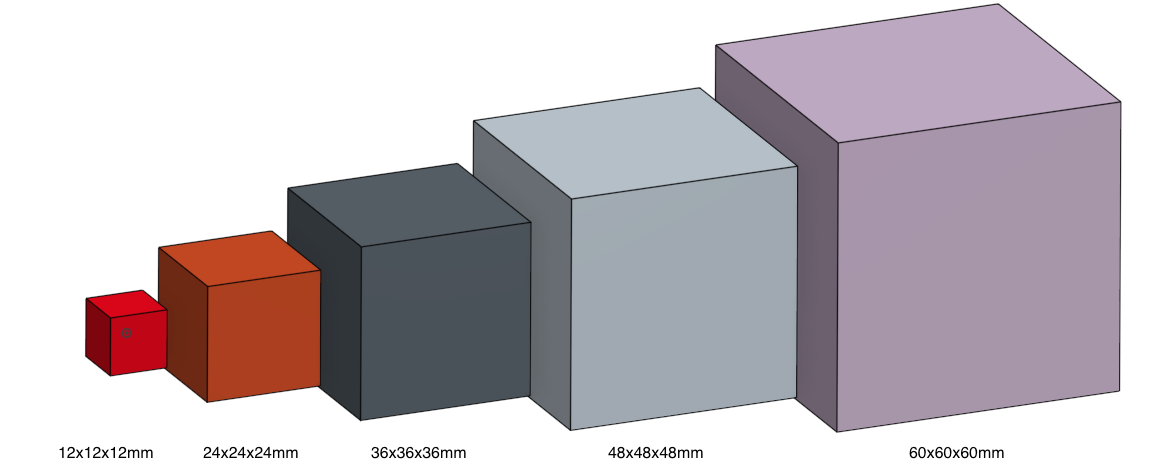
\includegraphics[width=0.8\columnwidth]{images/module_size.png}
    \end{center}
    \item \textbf{Pattern de fixation:} Sur chaque face d'un module se répète un pattern identique quelque soit la taille du module. Plusieurs patterns sont encore à l'étude.
\end{itemize}

De plus, la standardisation mécanique permet d'envisager la generation automatique de pièce mécanique permettant de fixer n modules entre eux. Pour ces aspects, des discussions sont en cours avec Sylvain Lefevbre (Inria Nancy) autour de ShapeForge.
}


\block{Mise en réseau}{

Pour simplifier le cablage du robot, nos modules sont mis en réseau et se connectent les uns aux autres. Quelque soit leur taille, ils partagent la même connectique, le même bus et peuvent être identifiés au démarrage du robot. Ils se voient alors attribuer une adresse relative à leur emplacement physique (voir schéma suivant). Il est alors possible d'enlever ou d'ajouter n'importe quel module et ce, n'importe où en le raccordant à un module voisin.

Le bus utilisé est un bus I2C ayant les propriétés suivantes:

\begin{itemize}
    \item \textbf{Multi-master:} Tous les modules peuvent communiquer entre eux. Il n'est pas necessaire d'avoir une gestion des comportements centralisés. Il devient alors possible d'imaginer la création de comportements emergents résultants de la somme d'ensemble de comportements simple et locaux, des reflexes par exemple.
    \item \textbf{Peu de fils:} Les cables sont l'un des éléments les moins fiables sur un robot. L'I2C nous permet de les minimiser en cablant l'ensemble du robot avec un réseau de 4 fils.
    \item \textbf{Rapide:} Avec la norme high speed, l'i2C peut être utilisé à 3,4Mbaud.
    \item \textbf{Souple:} L'aspect synchrone de l'I2C permet une compatibilité avec un grand nombe de système existant.
\end{itemize}

    % \begin{center}
    %     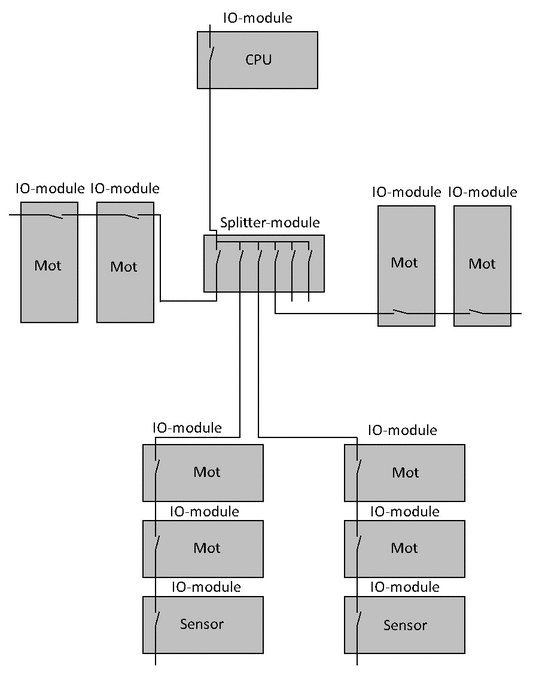
\includegraphics[width=0.7\columnwidth]{images/arch.png}
    % \end{center}

}


\block{Structure logiciel des modules}{

Comme pour la mécanique et la communication, les modules partagent une architecture logiciel commune:
\begin{itemize}
    \item \textbf{Bootloader:} La gestion de l'adressage dynamique et du démarrage sera inspiré du bootloader Arduino afin de garder la compatibilité avec cet environement.
    \item \textbf{Communication:} Une bibliothèque permettra de simplifier la communication entre les modules et sera accessible à tous les developpeurs.
    \item \textbf{Application:} Chaque module peut avoir sa propre application unique pour cela un espace de code dédié au module et au programme utilisateur sera aloué.
    % \vspace{1cm}
    \begin{tabular}{cc}
        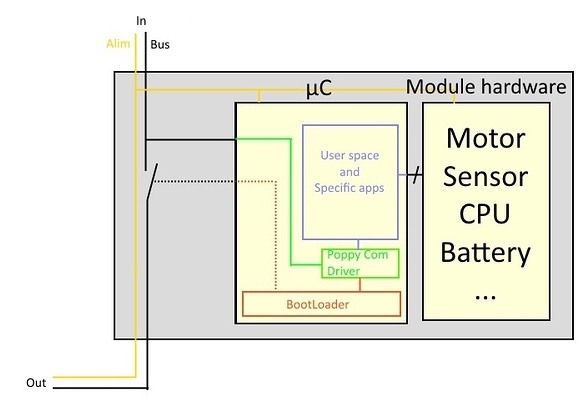
\includegraphics[width=0.45\columnwidth]{images/modul_arch.jpg} &
        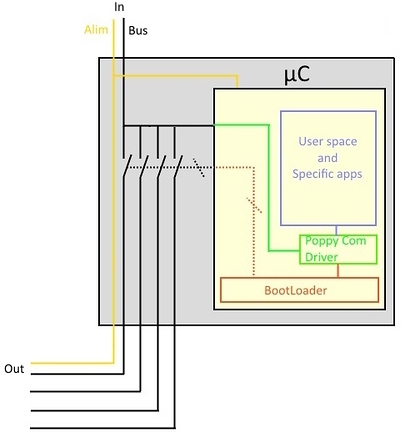
\includegraphics[width=0.45\columnwidth]{images/splitter_arch.jpg}
    \end{tabular}
\end{itemize}
}

\block{Structure logiciel haut niveau}{

L'interface sera la première vision de l'architecture, ainsi il est très important de bien comprendre les besoins :
\begin{itemize}
    \item \textbf{Librairie multilangage :} La bibliothèque de controle de Poppy pourra être utilisé avec différents langages.
    \item \textbf{Programmation visuelle :} Poppy 2.0 sera compatible avec Snap.
    \item \textbf{Application web :} Un IDE sur le navigateur.
    \item \textbf{Compatibilité :} Tous les contenus pédagogique développé pour Poppy 1 resteront compatible avec l'architecture Poppy 2.0.
\end{itemize}
}


\block{Module Open source actuator}{

Sur un robot, les actuateurs sont actuellement l'element limitant et limité, il s'agit pourtant d'un élément fondamental. L'utilisation de servo-moteurs Robotis très couteux est un frein pour la diffusion des créatures Poppy 1. Il est ainsi absolument critique de réussir à proposer une alternative à la fois open source, accessible et de très bonne qualité.

Ces modules moteurs s'integreront dans l'architecture (mecanique, communication, logiciel) présentés précédement:

\begin{center}
        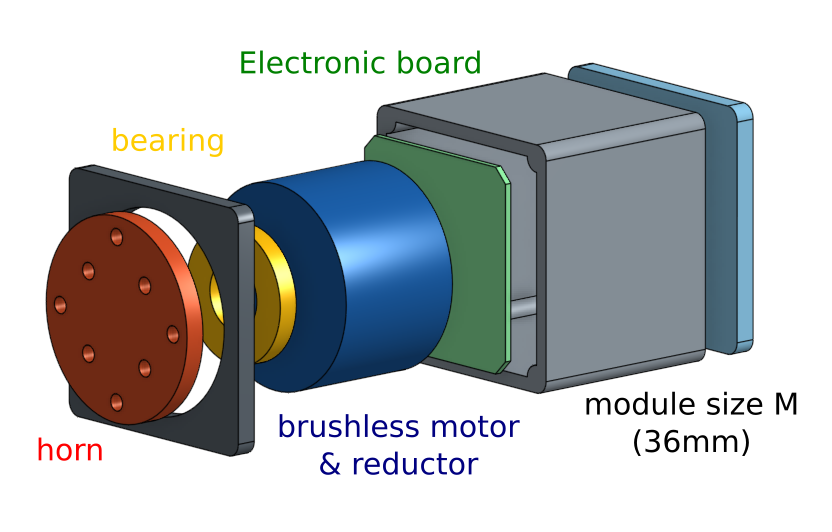
\includegraphics[width=0.6\columnwidth]{images/module_moteur.png}
\end{center}

D'un point de vue technique, ils s'inspirent des travaux du MIT sur l'"optimal Actuator" en proposant une transmission faible impédance et haute densité de couple, permettant un contrôle en force précis.

}

\block{Planning}{
\begin{tabular}{|c|c|}
    \hline
        \textbf{jalon} & \textbf{date} \\
    \hline
        Définition des technologies et des besoins : & mai 2015 \\
        Réalisation de la carte processeur : & aout 2015 \\
        Test des API mécanique sur un cas concret : & octobre 2015 \\
        Réalisation d'un prototype de moteur : & janvier 2016 \\
        Test et validation d'une gamme de moteur : & avril 2016 \\
        Création d'autres modules autour d'une application concrète : & juin 2016 \\
        Dissémination de la technologie : & sept 2016 \\
        transfert vers une structure : & sept 2016 \\
    \hline
\end{tabular}

}


% \block{References}
% {
% 	% \vspace{-10pt}
% 	\nocite{*}
% 	\bibliographystyle{abbrv}
% 	\renewcommand{\section}[2]{}% Hack to remove bibliography title
% 	\bibliography{ref}
% 	\vspace{-10pt}
% }

\end{multicols}
% \vfill
\end{document}
